\section{STRATEGY AND BATTLE ORDER}
\hfill

GENERAL RULE:

In the Order Phase of every Battle Turn, each player selects a basic strategy for each wing or nationality in his army for the ensuing Battle Turn. The Order Tables simulate the general inefficiency and lack of control that plagued medieval commanders.

\subsection{Wings and Nationalities}

Each player's army is divided into \textit{wings} (Saxons) or \textit{nationalities} (Normans) for determining battle order. Norman nationalities are further divided into \textit{sections} of foot and knights.

\subsubsection[Saxon Wings]{}

The Saxon Army initially consists of three wings - right, center and left - each commanded by a leader. The leader's command radius usually determines which units make up his wing.

\subsubsection[Defining Saxon Wings]{}

Wings are defined at the beginning of each individual Battle Turn. No Saxon leader can control less than 20\% (1/5) of the Saxon units available. A given leader can control any number of units within his command radius as long as no Saxon leader controls less than 20\% of the Saxon units.

\subsubsection[Saxon Leader Loss and Wings]{}

If the Saxons are reduced to less than three leaders, no leader can control less than 33\% (1/3) of the Saxon units. If a Saxon leader dies during a Battle Turn, his wing is what it originally was until its units come under the control of the remaining Saxon leaders. If the Saxons have no leaders, they are assumed to have only one wing.

\subsubsection[Norman Sections]{}

The Norman army has six sections: Norman Foot/Bowmen, Norman Knights, Breton Foot/Bowmen, Breton Knights, Franco-Flemish Foot/Bowmen, and Franco-Flemish Knights. William's personal guard is \textit{not} part of any section (see 4.38). Norman leaders do not define Norman sections.

\subsubsection[Leaders and Unit Orders]{}

Leaders never affect the order of their units. An army can operate without leaders, albeit with reduced efficiency.

\subsubsection[Define Wings and Sections]{}

Players must always clearly define their wings and sections. Certain situations can make this difficult. Try to establish what is what before you proceed, and treat this rules section liberally in that respect.

\subsection{Strategy}

Specific strategies are chosen for each wing or nationality for each Battle Turn. These will influence, but not control, the order adopted by the units of the wing or sections of the nationality for the turn (medieval troops were notoriously difficult to control). The strategy used will have a long-term effect on friendly morale and endurance.

\subsubsection[Strategies]{}

There are four strategies available: Defensive, Cautious, Moderate, and Aggressive. The player can choose a different (or the same) strategy for each of his wings or nationalities. Each player has a number of Strategy markers corresponding to the available strategies.

\subsubsection[Strategy Display]{}

Each player has a Strategy Display on the game map. In the Order Phase of each Battle Turn, the player places face-down in each box a Strategy marker corresponding to his selected strategy for that wing or nationality. The strategies are not revealed until the players are ready to determine their battle order.

\subsubsection[Order Tables]{}

After a strategy has been chosen for each wing/nationality, the players consult the Order Tables printed on the map. Each player rolls two dice for each wing/nationality and compares the roll to the strategy selected for that wing/nationality to find out what order it will adopt during the ensuing Battle Turn. The order rolled is applied to all units in that wing or section (see 4.24). An Order Marker is placed in the appropriate box on the player's Order Display (printed on the map), indicating the order in effect for the turn. The Morale marker for that wing or section is adjusted on the Strategy Effects Table.

\textcolor{blue}{When determining the Norman Strategy Effect from the Battle Order Determination Table (4.46) the separate effects of the Knights and the Foot are combined (i.e. they are cumulative) for a given nationality. Thus a -2 and a +1 would produce an effect for that turn of -1.}

\subsubsection[Orders]{}

The Saxon player rolls for each existing wing. The Norman player rolls for each \textit{nationality} (Norman, Breton, and Franco-Flemish). \textbf{Important:} This roll is read separately for both the knight and foot units of their nationality.

\subsubsection[Leaders and Orders]{}

Leaders never adopt an order; they are not affected by these rules.

\subsubsection[Order Length]{}

Some orders last for two turns. Wings/sections in those orders ignore theorder dice roll. Instead, their marker is moved from the "2" turn box to the "1" turn box on the player's Order Display.

\subsubsection[Optional Order]{}

A result of \textbf{Optional} means that the player chooses the order desired for that wing/section for the phase.

\subsection{Battle Order}

\textit{The following battle order descriptions (4.31 through 4.34) are adopted only by foot units.}

\subsubsection{Shield Wall:} Non-bow foot units in this order use their \textit{Shield Wall} combat strengths. They are not required to attack (an exception to 8.12). Their movement allowance is "0"; however, units using thsi order can move one hex towards the rear (9.23) as long as they do not enter an enemy zone of control. Units in Shield Wall order cannot "react" as per 5.4.

Bowmen never adopt a Shield Wall order; if this order is in effect, bowmen (only) adopt Melee/Fire in Place instead.

\subsubsection{Melee/Fire in Place:} Units use their normal combat strengths and can fire and melee normally. Units in this order have a movement allowance of "0", but may either advance or retreat one hex as long as they do not enter an enemy zone of control.

\subsubsection{Advance to Combat:} All combat strengths and movement allowances are normal and unrestricted. Movement is voluntary for each unit Units need not move toward the enemy.

\subsubsection{Attack \& Pursue \textit{(Saxon foot only)}:} Any unit in this order must, where possible, move toward the nearest enemy unit. Units in this order not adjacent to the enemy must move as close to such units as possible; those in an enemy zone of control can move, so long as they end their movement adjacent to an enemy unit. In addition:

\begin{itemize}
  \item Units in this order cannot move in the friendly reaction segment.
  \item During melee, normal combat strengths are used. \textbf{D} combat results inflicted by units in this order become \textbf{R} results. Units in this order routing an enemy unit \textit{must} pursue, as detailed in Case 9.4.
  \item The Attack \& Pursue order remains in effect for the number of Battle Turns given on the Order Table.
\end{itemize}

\textit{The following orders are adopted only by Norman knights of any nationality:}

\subsubsection{Hold:} This is the same as the Shield Wall order, except that the knights use their normal combat strength.

\subsubsection{Advance:} This is the same as 4.33.

\subsubsection{Charge:} This is a voluntary order that allows knight units to increase their combat strengths under certain conditions. If the conditions cannot be met, or if the Norman player does not wish to charge, the individual knight unit will be in the Advance to Combat order. Charge conditions are:

\begin{itemize}
  \item The charge must end in contact with an enemy unit.
  \item The charge cannot cross a ridge or stream hexside, or enter a marsh or woods hex.
  \item The last two hexes of the charge cannot be uphill (see 5.33).
\end{itemize}

When charging, knights have a movement allowance of \textit{six} and all knight units in the section (whether actually charging or not) must move toward the enemy, as described in 4.34. In addition:

\begin{itemize}
  \item Units in this order cannot move in a friendly reaction segment.
  \item In melee, a successfully charging knight unit adds \textit{one} to its combat strength; \textit{two} if charging downhill.
  \item All \textbf{D} results inflicted by charging knights are treated as \textbf{R} results (see 9.1). After a successful charge (and subsequent melee) the knight unit must undergo a morale check (see 9.62) regardless of any other combat result. Routed enemy units must be pursued by undisrupted knights as per 9.4.
  \item A Charge order remains in effect for the number of turns given on the Order Table.
\end{itemize}

\textcolor{blue}{If a Knight unit receives a Charge order, but does not meet the conditions for Charging (the three conditions listed at the beginning of the section), it may still increase its movement rate (to 6 MPs); however, if it attacks, it uses its printed attack strength (it does not receive the +1/+2 Charge bonus). All other effects apply, however, as if the Charge were allowed.}

\subsubsection[Exceptions to Order Rules]{} The following situations are exceptions to the order rule:

\begin{enumerate}
  \item \textbf{William's Guard:} This knight unit (distinguished by its "A" morale) is free to move as desired by the Norman player - as long as William is alive. It is not affected by the order rules and may charge at any time, as long as it meets the charge requirements. If William is dead, the unit becomes part of the Norman knight section.
  \item \textbf{Saxon Reinforcements:} When entering the game as per 12.3, these units are in Advance to Combat order until they come within the command radius of a leader \textit{or} move adjacent to an enemy unit. At this point they are arbitrarily assigned to the nearest wing.
  \item \textbf{Harold's Housecarls (optional rule):} Historically the Saxon housecarls were less impetuous than the fyrd, who tended to charge recklessly into combat. Thus, the housecarls treat an Attack \& Pursue order as an Optional order. The Saxon player, however, must make this decision prior to his order dice roll and cannot change his mind after the roll is made. \textit{(This rule greatly favors the Saxons and can be used as a balancing element)}
\end{enumerate}

\subsection{Displays and Tables}

\subsubsection{Saxon Strategy Display}

\begin{center}
  \begin{noverticalspace}
    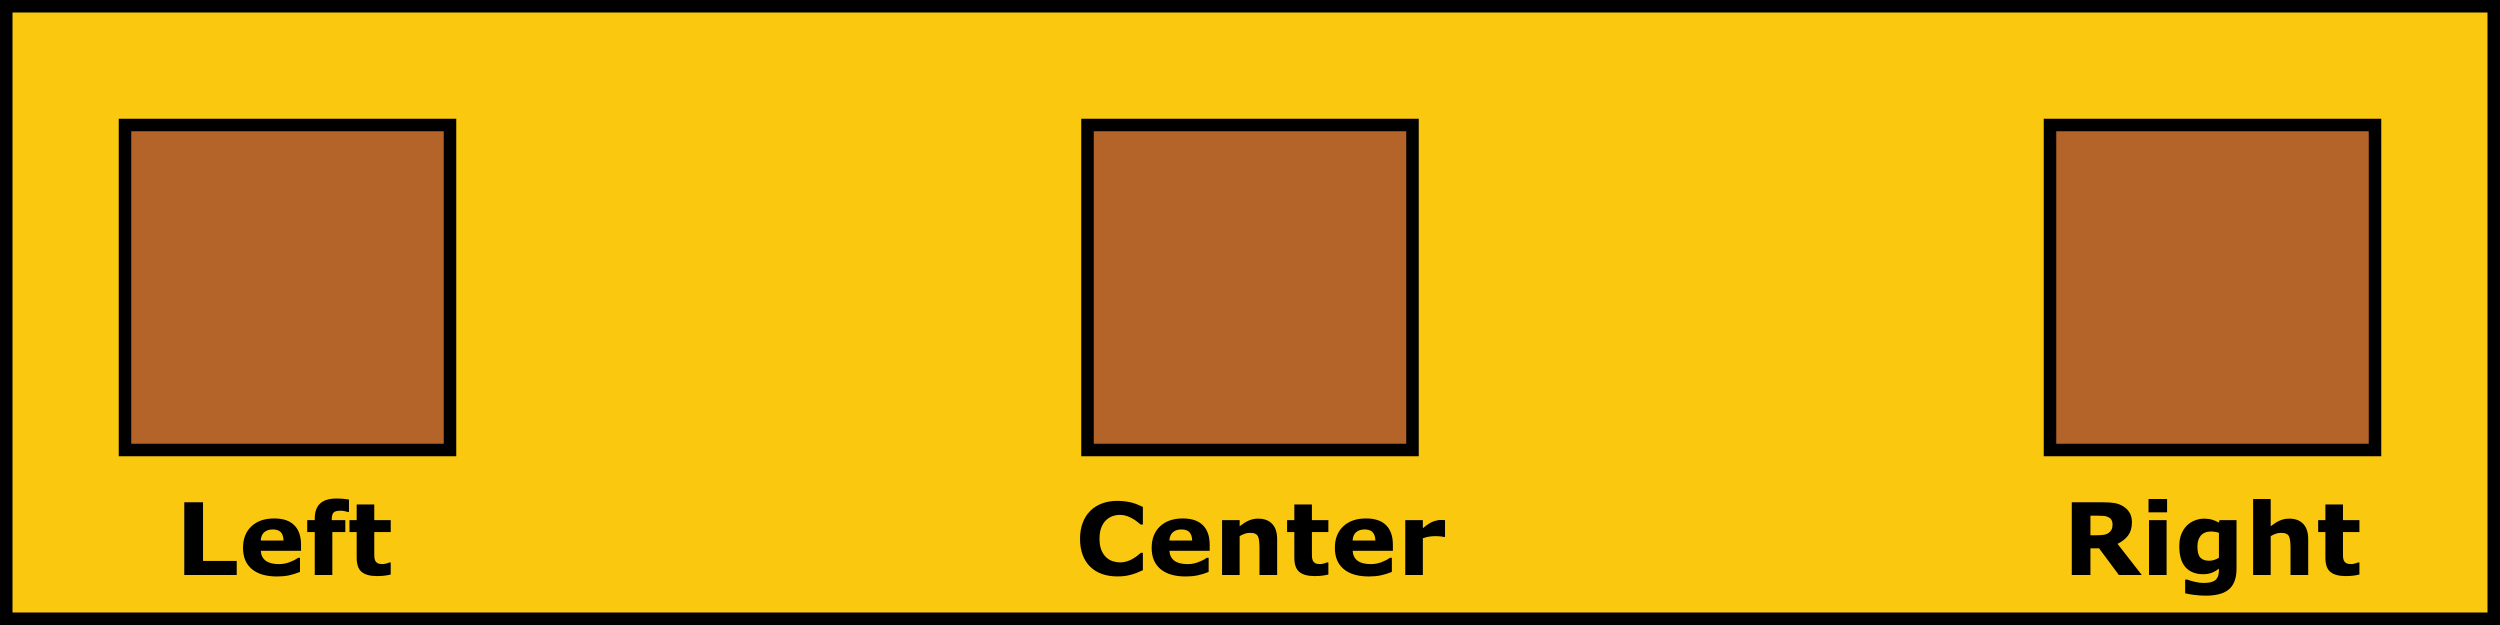
\includegraphics[scale=0.75]{Saxon_Strategy_Display.png}
  \end{noverticalspace}
\end{center}

\subsubsection{\mbox{Saxon Battle Order Determination Table}}

\begin{center}
  \begin{noverticalspace}
    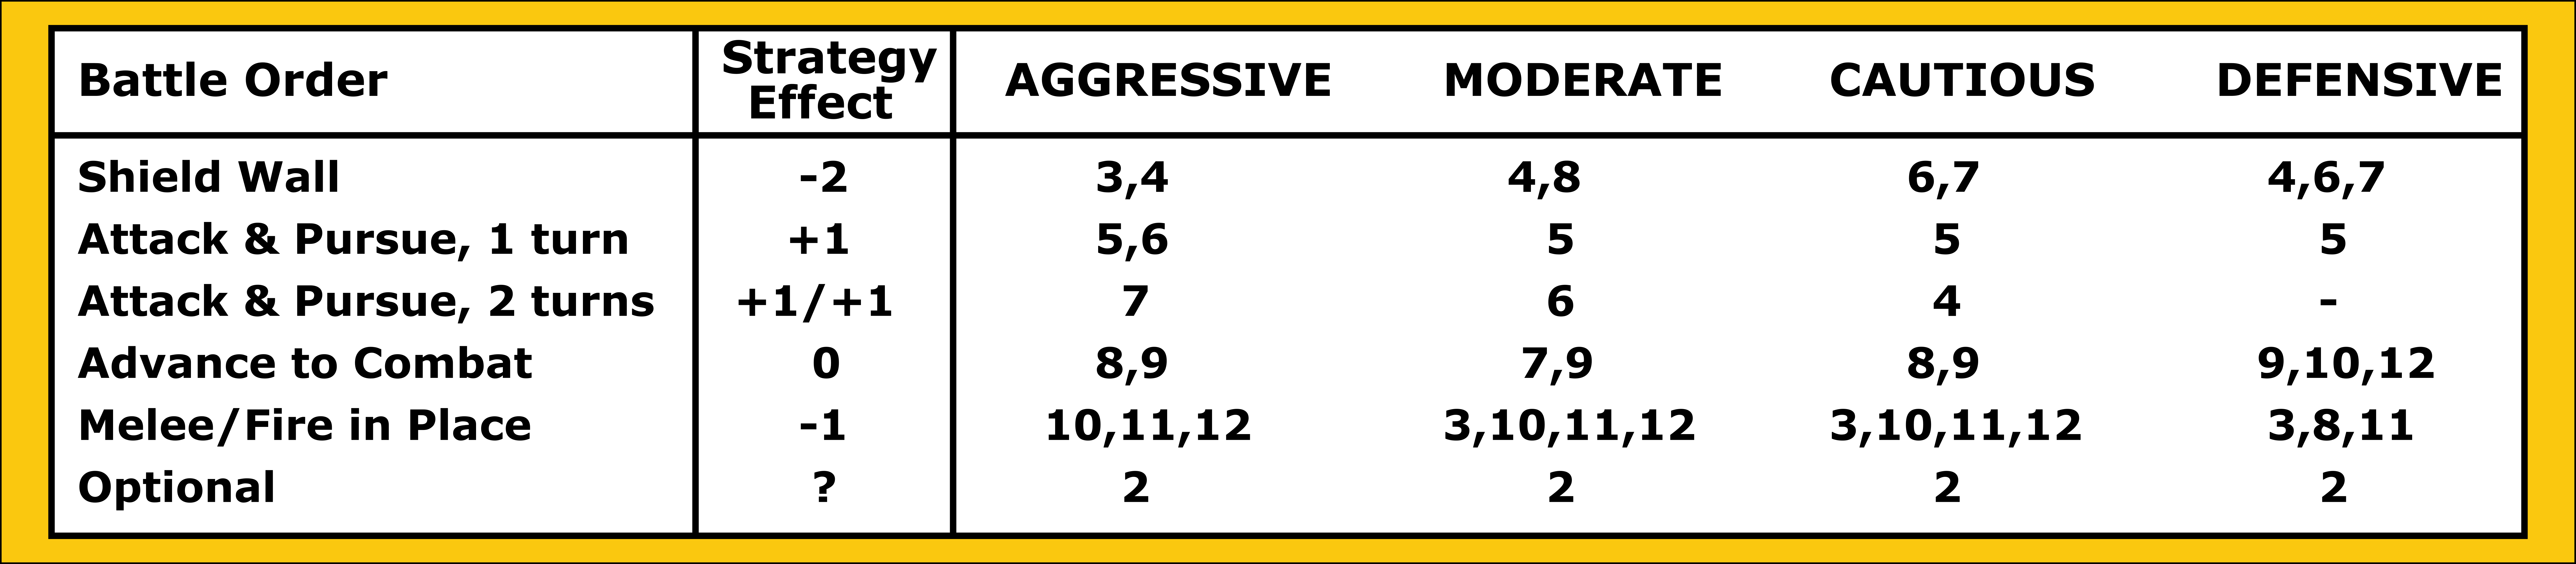
\includegraphics[scale=0.48]{Saxon_Battle_Order_Determination_Table.png}
  \end{noverticalspace}
\end{center}

\subsubsection{Saxon Battle Order Display}

\begin{center}
  \begin{noverticalspace}
      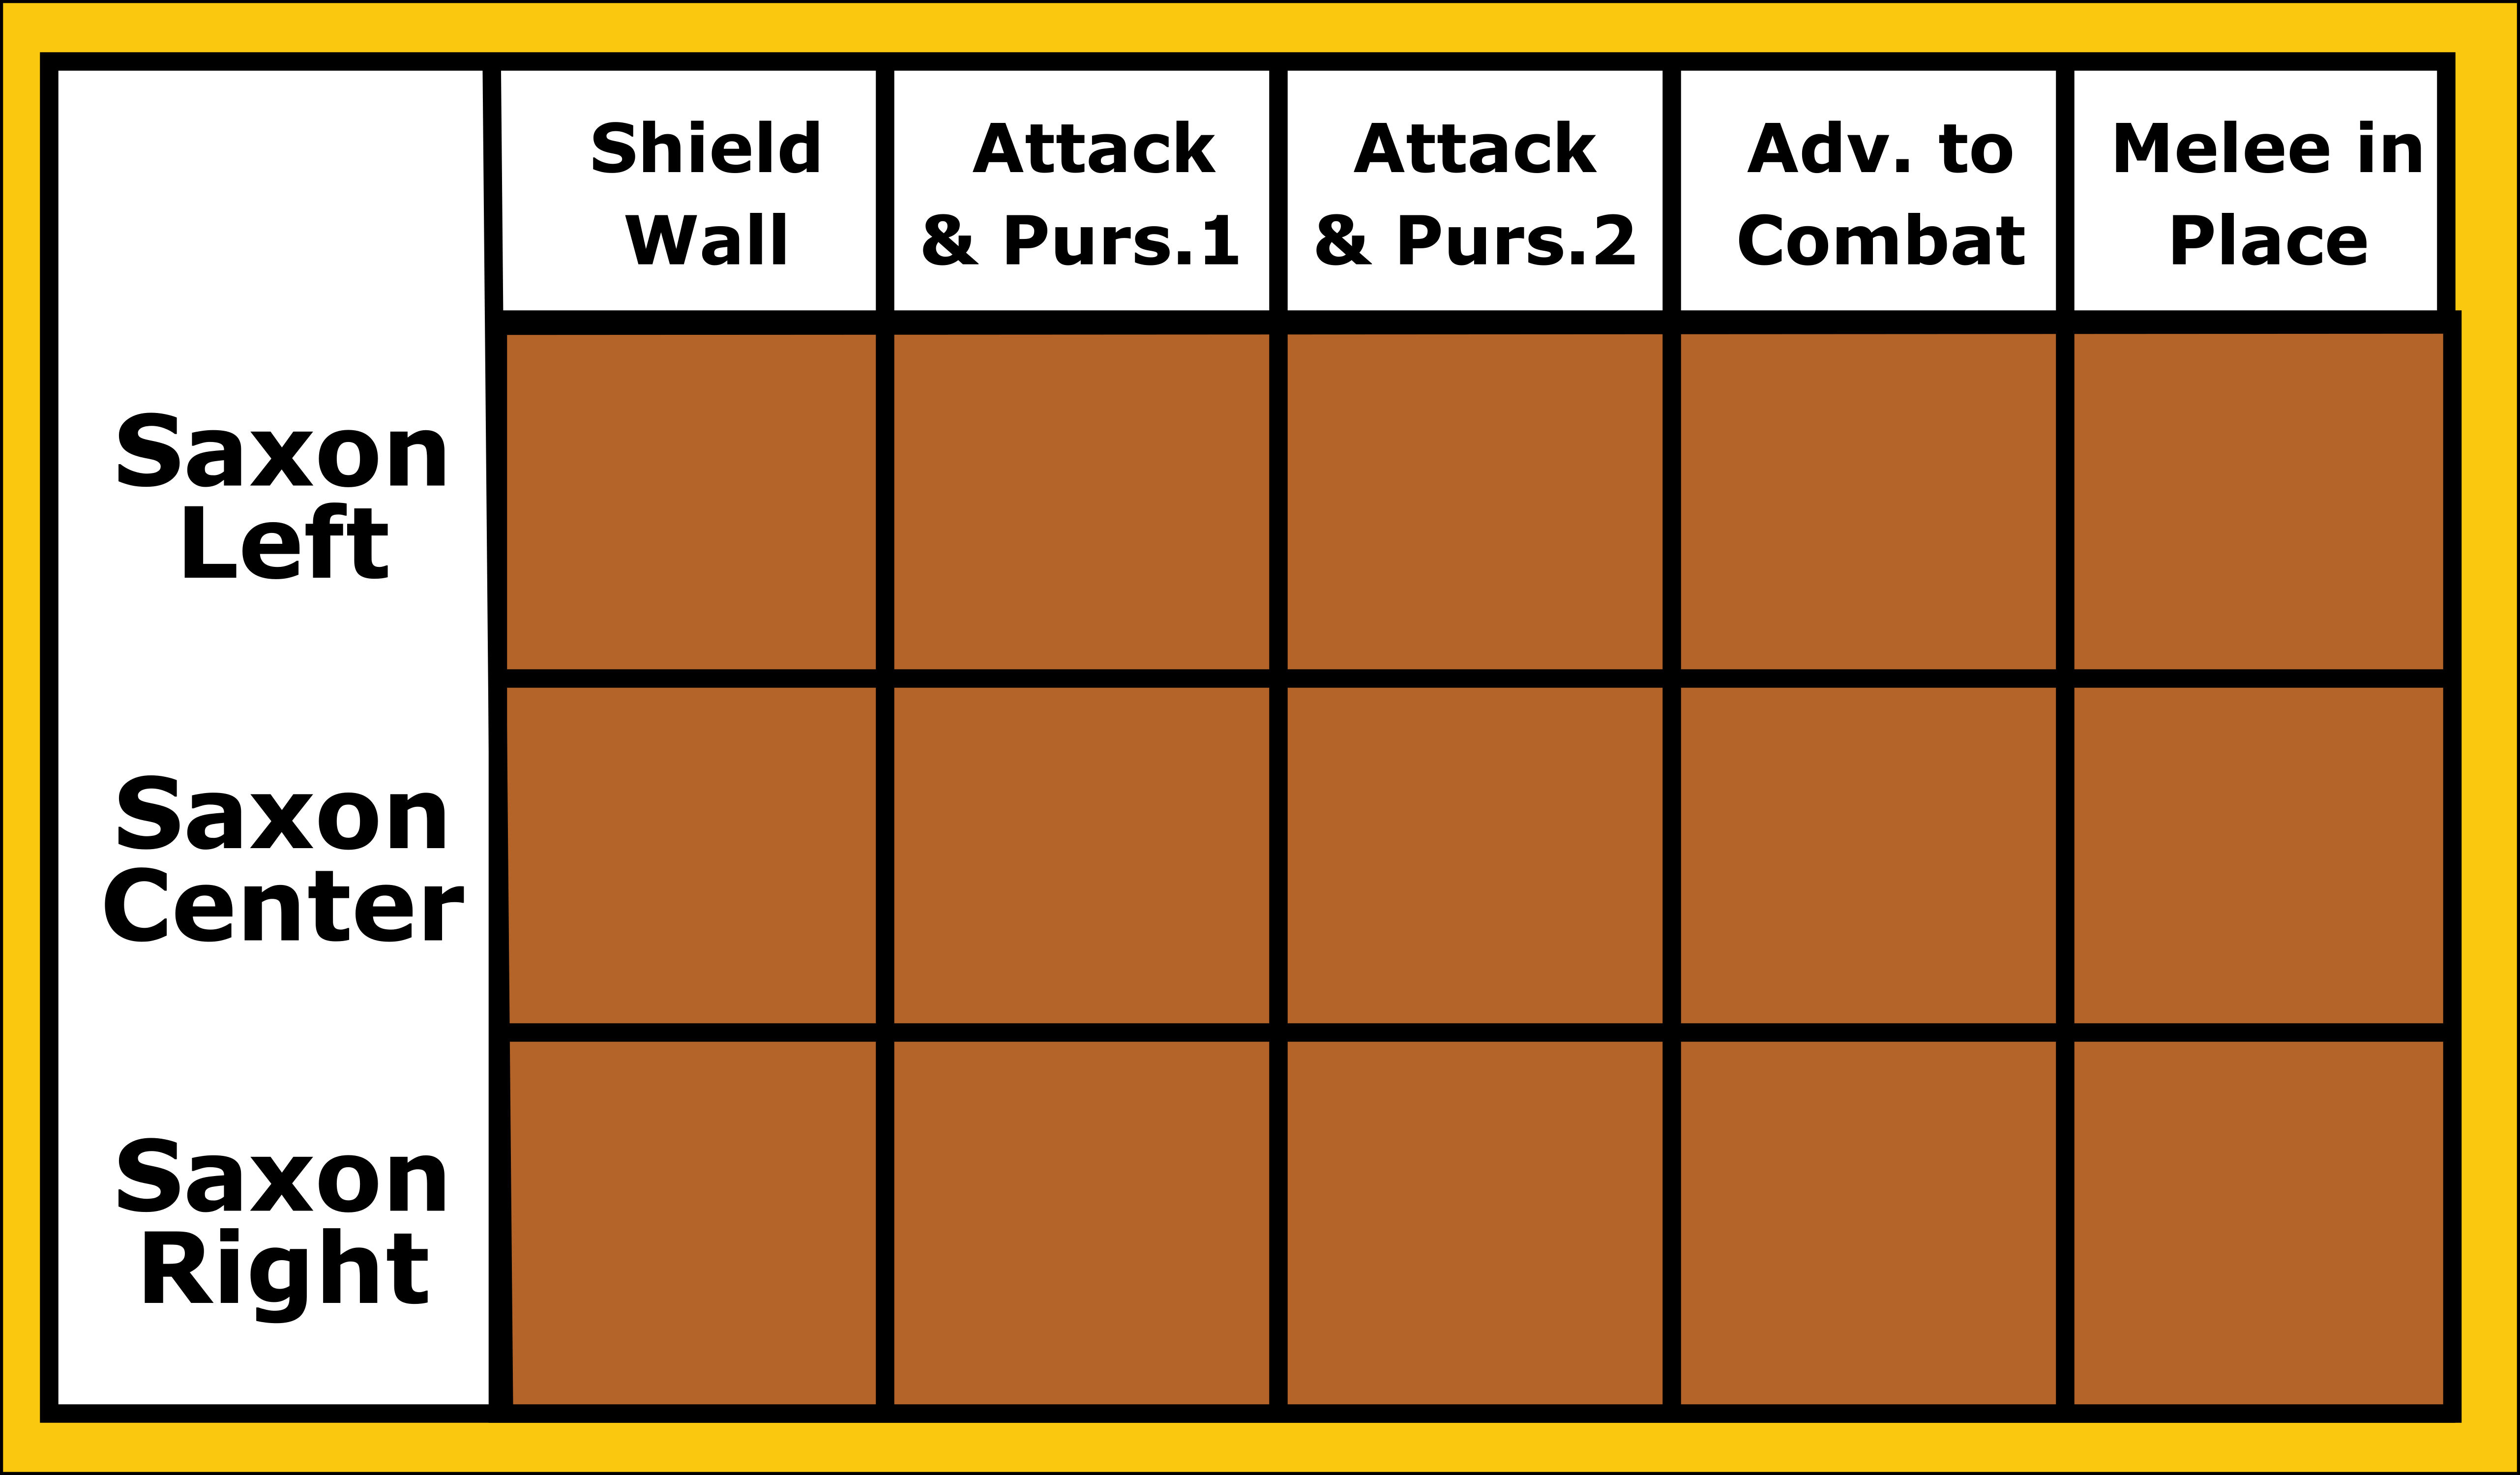
\includegraphics[scale=0.40]{Saxon_Battle_Order_Display.png}
  \end{noverticalspace}
\end{center}

\subsubsection{Saxon Strategy Effects Track}

\begin{center}
  \begin{noverticalspace}
    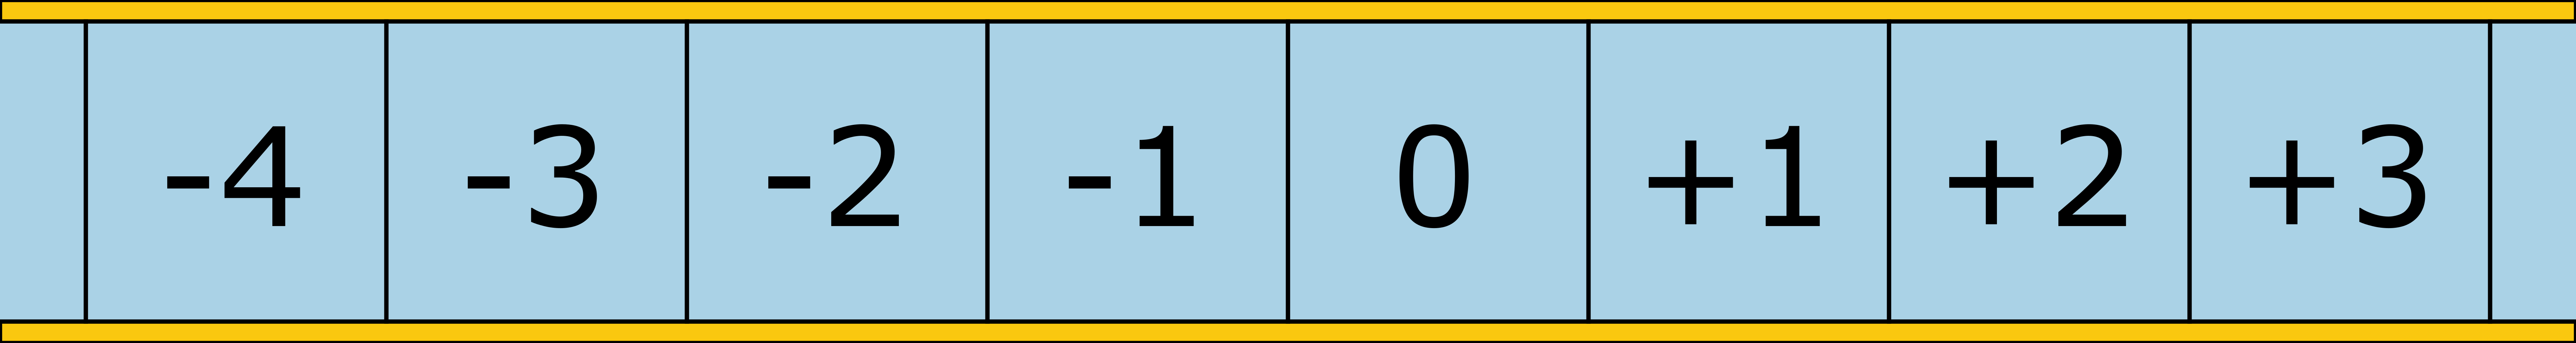
\includegraphics[scale=0.40]{Saxon_Strategy_Effects_Track.png}
  \end{noverticalspace}
\end{center}

\subsubsection{Norman Strategy Display}

\begin{center}
  \begin{noverticalspace}
    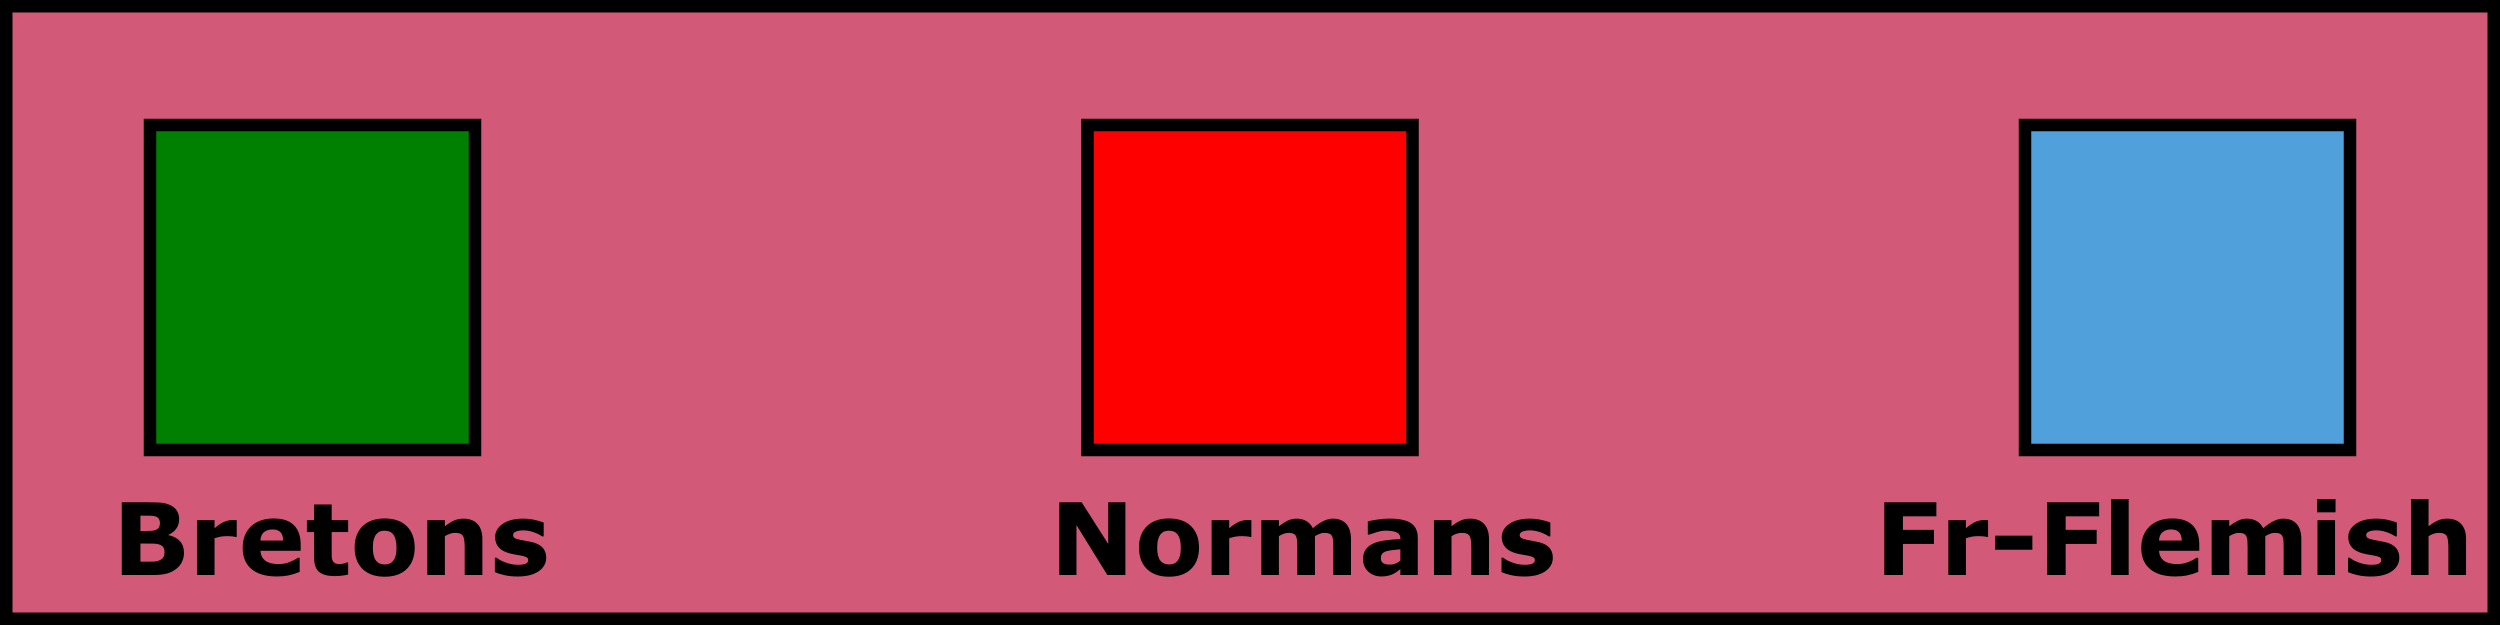
\includegraphics[scale=0.75]{Norman_Strategy_Display.png}
  \end{noverticalspace}
\end{center}

\subsubsection{Norman Battle Order Determination Table}

\subsubsection{Norman Battle Order Display}

\subsubsection{Norman Strategy Effects Track}

\begin{center}
  \begin{noverticalspace}
    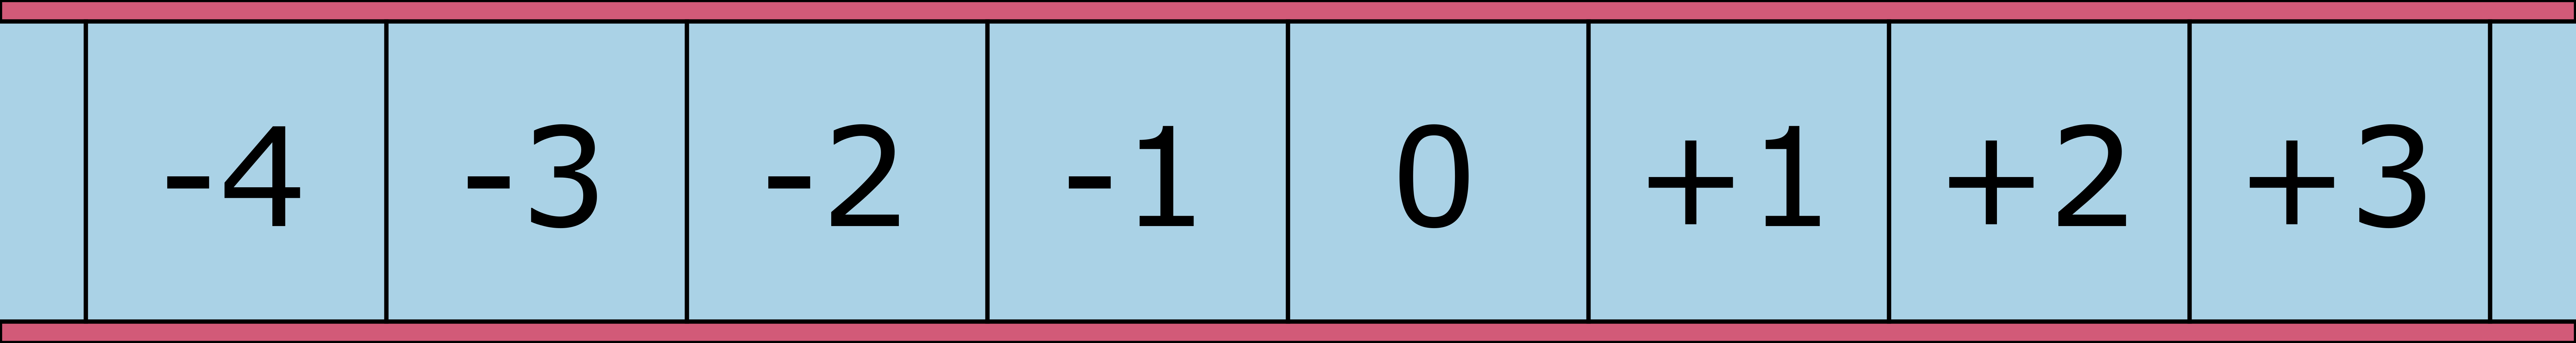
\includegraphics[scale=0.40]{Norman_Strategy_Effects_Track.png}
  \end{noverticalspace}
\end{center}

\hfill

\textcolor{blue}{At the beginning of the game, all ratings on the Strategy Effects Track start at "0". Additionally, at the start of the second Assault Period, return all ratings back to "0".}
